\documentclass[11pt]{scrartcl}
\usepackage[T1]{fontenc}
\usepackage[a4paper, left=3cm, right=2cm, top=2cm, bottom=2cm]{geometry}
\usepackage[activate]{pdfcprot}
\usepackage[ngerman]{babel}
\usepackage[parfill]{parskip}
\usepackage[utf8]{inputenc}
\usepackage{kurier}
\usepackage{amsmath}
\usepackage{amssymb}
\usepackage{xcolor}
\usepackage{epstopdf}
\usepackage{txfonts}
\usepackage{fancyhdr}
\usepackage{graphicx}
\usepackage{prettyref}
\usepackage{hyperref}
\usepackage{eurosym}
\usepackage{setspace}
\usepackage{units}
\usepackage{eso-pic,graphicx}
\usepackage{icomma}
\usepackage{pdfpages}

\definecolor{darkblue}{rgb}{0,0,.5}
\hypersetup{pdftex=true, colorlinks=true, breaklinks=false, linkcolor=black, menucolor=black, pagecolor=black, urlcolor=darkblue}



\setlength{\columnsep}{2cm}


\newcommand{\arcsinh}{\mathrm{arcsinh}}
\newcommand{\asinh}{\mathrm{arcsinh}}
\newcommand{\ergebnis}{\textcolor{red}{\mathrm{Ergebnis}}}
\newcommand{\fehlt}{\textcolor{red}{Hier fehlen noch Inhalte.}}
\newcommand{\betanotice}{\textcolor{red}{Diese Aufgaben sind noch nicht in der Übung kontrolliert worden. Es sind lediglich meine Überlegungen und Lösungsansätze zu den Aufgaben. Es können Fehler enthalten sein!!! Das Dokument wird fortwährend aktualisiert und erst wenn das \textcolor{black}{beta} aus dem Dateinamen verschwindet ist es endgültig.}}
\newcommand{\half}{\frac{1}{2}}
\renewcommand{\d}{\, \mathrm d}
\newcommand{\punkte}{\textcolor{white}{xxxxx}}
\newcommand{\p}{\, \partial}
\newcommand{\dd}[1]{\item[#1] \hfill \\}

\renewcommand{\familydefault}{\sfdefault}
\renewcommand\thesection{}
\renewcommand\thesubsection{}
\renewcommand\thesubsubsection{}


\newcommand{\themodul}{Optische Technologie}
\newcommand{\thetutor}{Prof. Rateike}
\newcommand{\theuebung}{Übung 2}

\pagestyle{fancy}
\fancyhead[L]{\footnotesize{C. Hansen}}
\chead{\thepage}
\rhead{}
\lfoot{}
\cfoot{}
\rfoot{}

\title{\themodul{}, \theuebung{}, \thetutor}


\author{Christoph Hansen \\ {\small \href{mailto:chris@university-material.de}{chris@university-material.de}} }

\date{}


\begin{document}

\maketitle

Dieser Text ist unter dieser \href{http://creativecommons.org/licenses/by-nc-sa/4.0/}{Creative Commons} Lizenz veröffentlicht.

\textcolor{red}{Ich erhebe keinen Anspruch auf Vollständigkeit oder Richtigkeit. Falls ihr Fehler findet oder etwas fehlt, dann meldet euch bitte über den Emailkontakt.}

\tableofcontents


\newpage

\section{Aufgabe 1}


\begin{figure}[h]
	\centering
	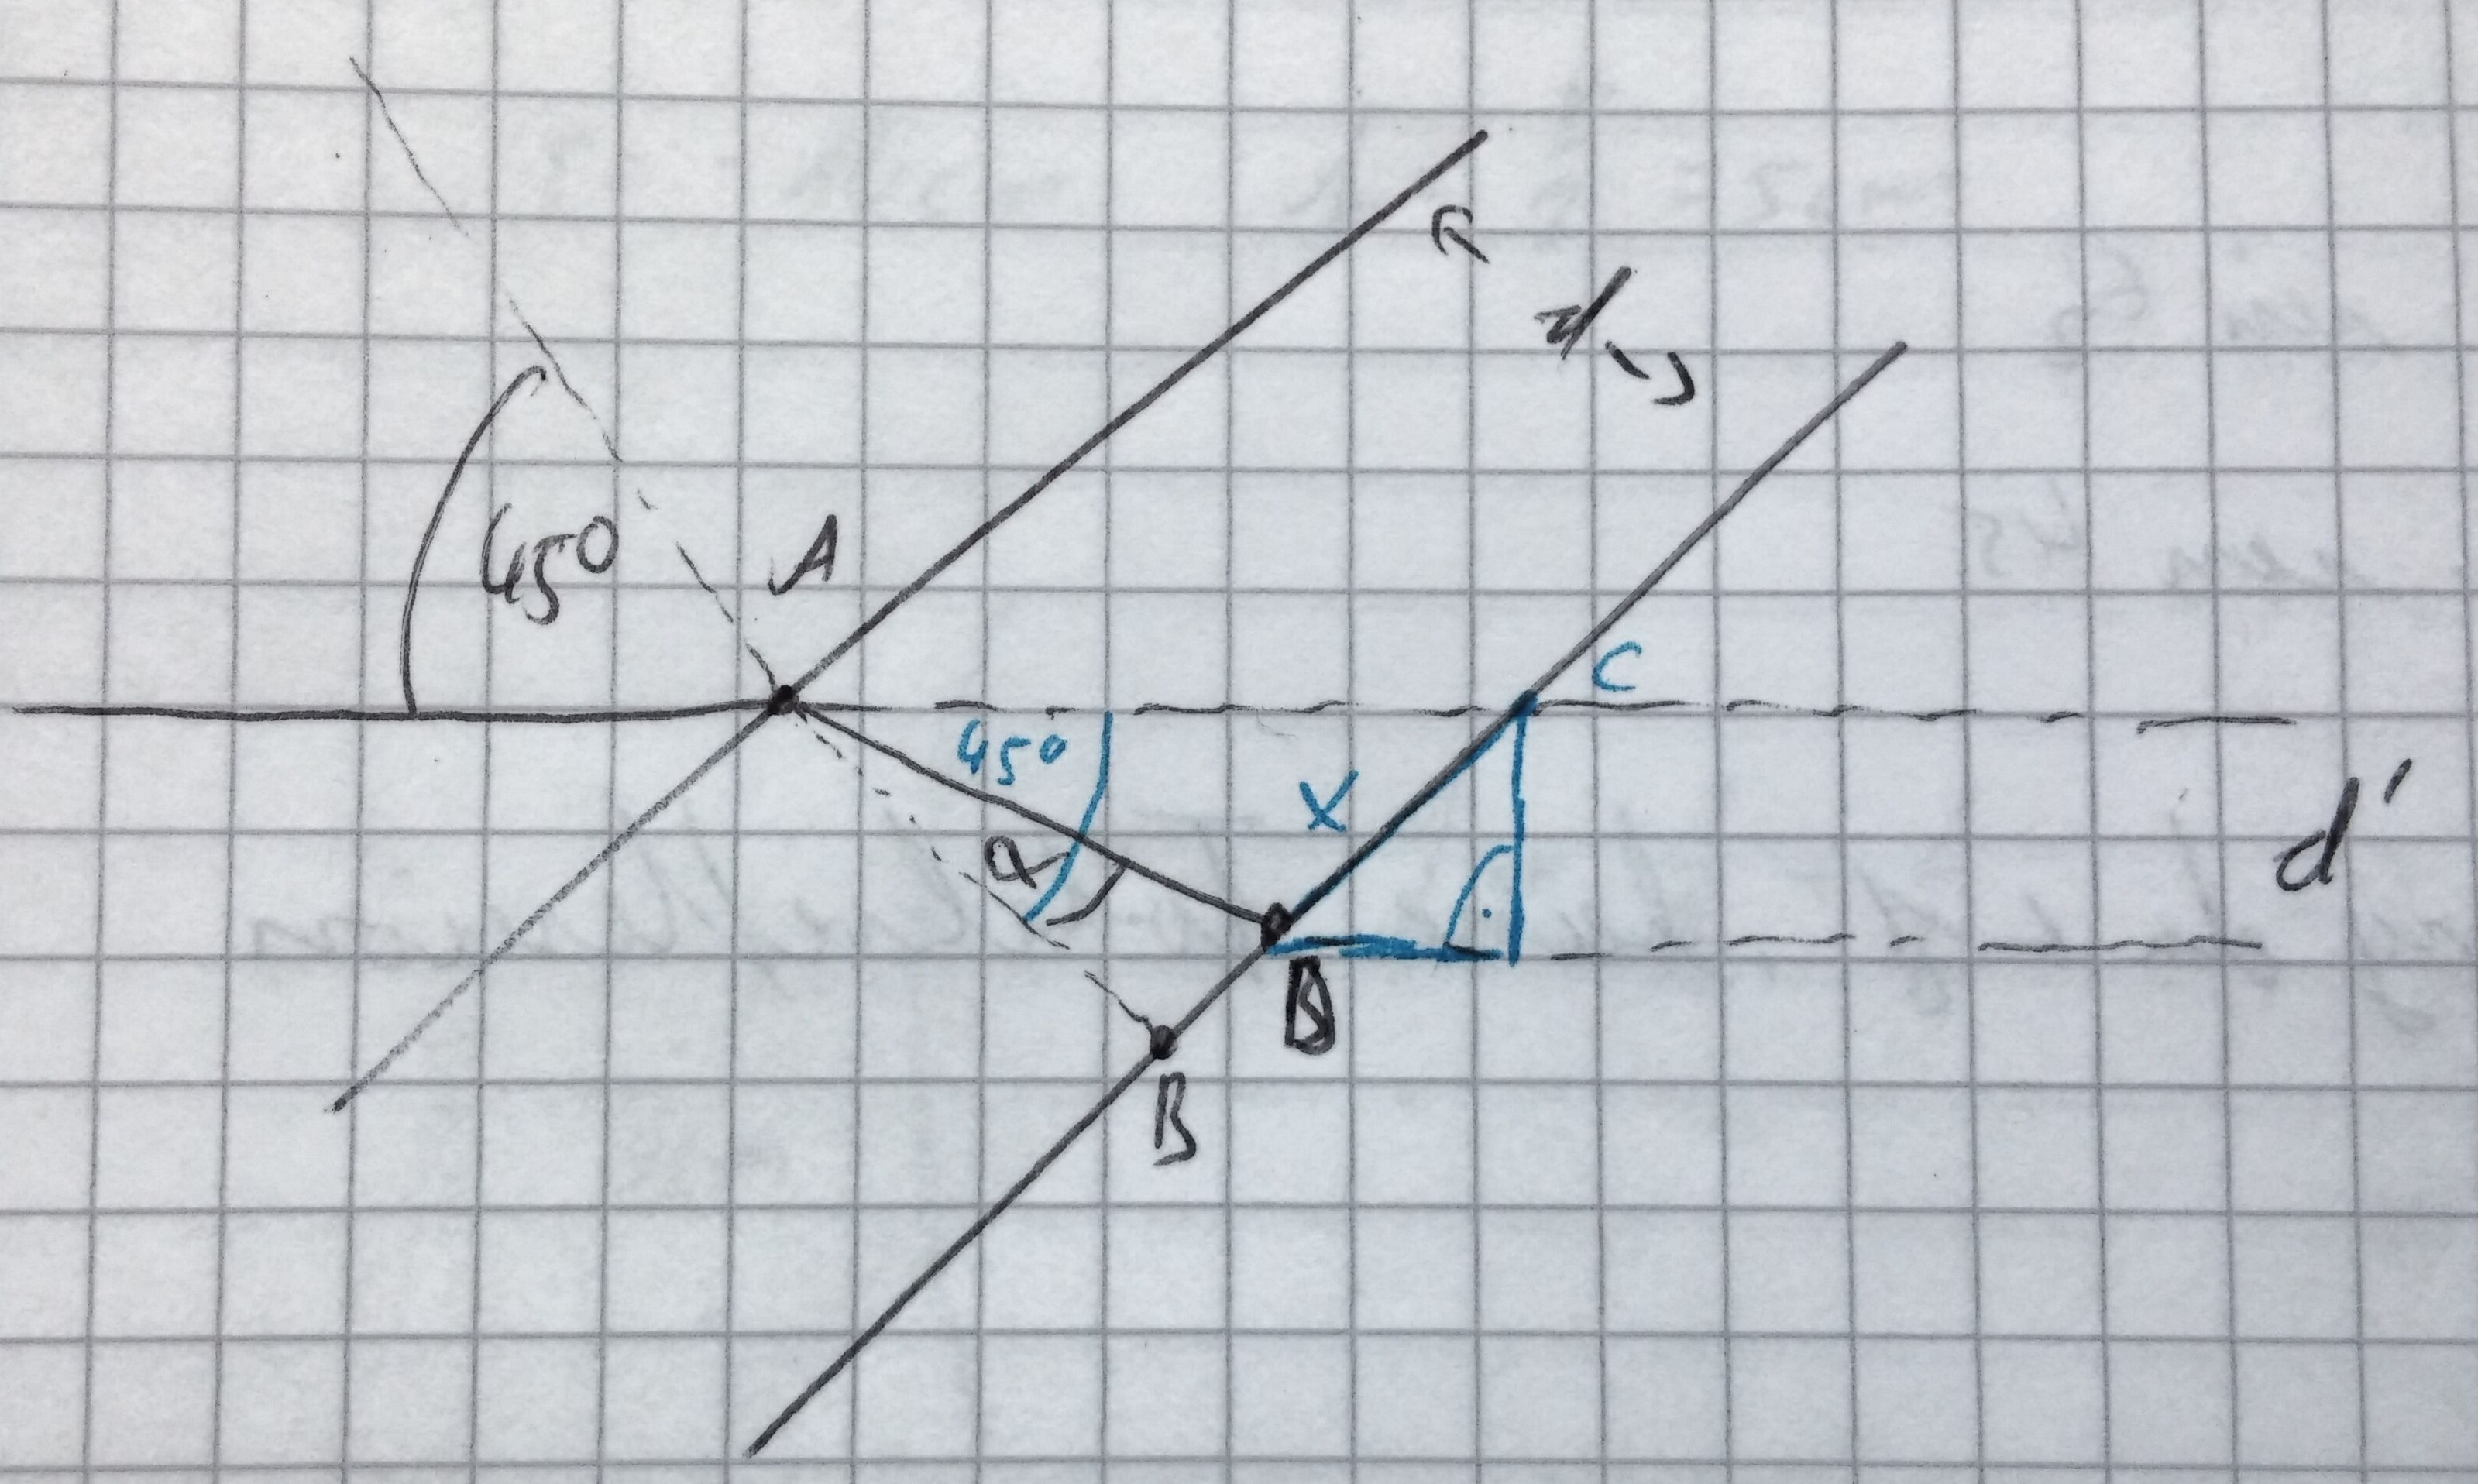
\includegraphics[scale=0.08]{A1_1.jpg}
\end{figure}

Das Dreieck $\Delta ABC$ ist gleichschenklig. Zudem gelten für die Strecken:

\begin{align*}
\bar{BC} &= d = \bar{AB} \\
\bar{BD} &= d \cdot \tan(\alpha) 
\intertext{Daraus folgern wir:}
x &= d - d \cdot \tan(\alpha) \qquad \text{mit} \qquad \sin(45) = n \cdot \sin(n) \Leftrightarrow \alpha = \arcsin\left( \frac{\sin(\alpha)}{n} \right) \\
\Rightarrow d' &= x \cdot sin(45)
\end{align*}


\section{Aufgabe 2}

\begin{figure}[h]
	\centering
	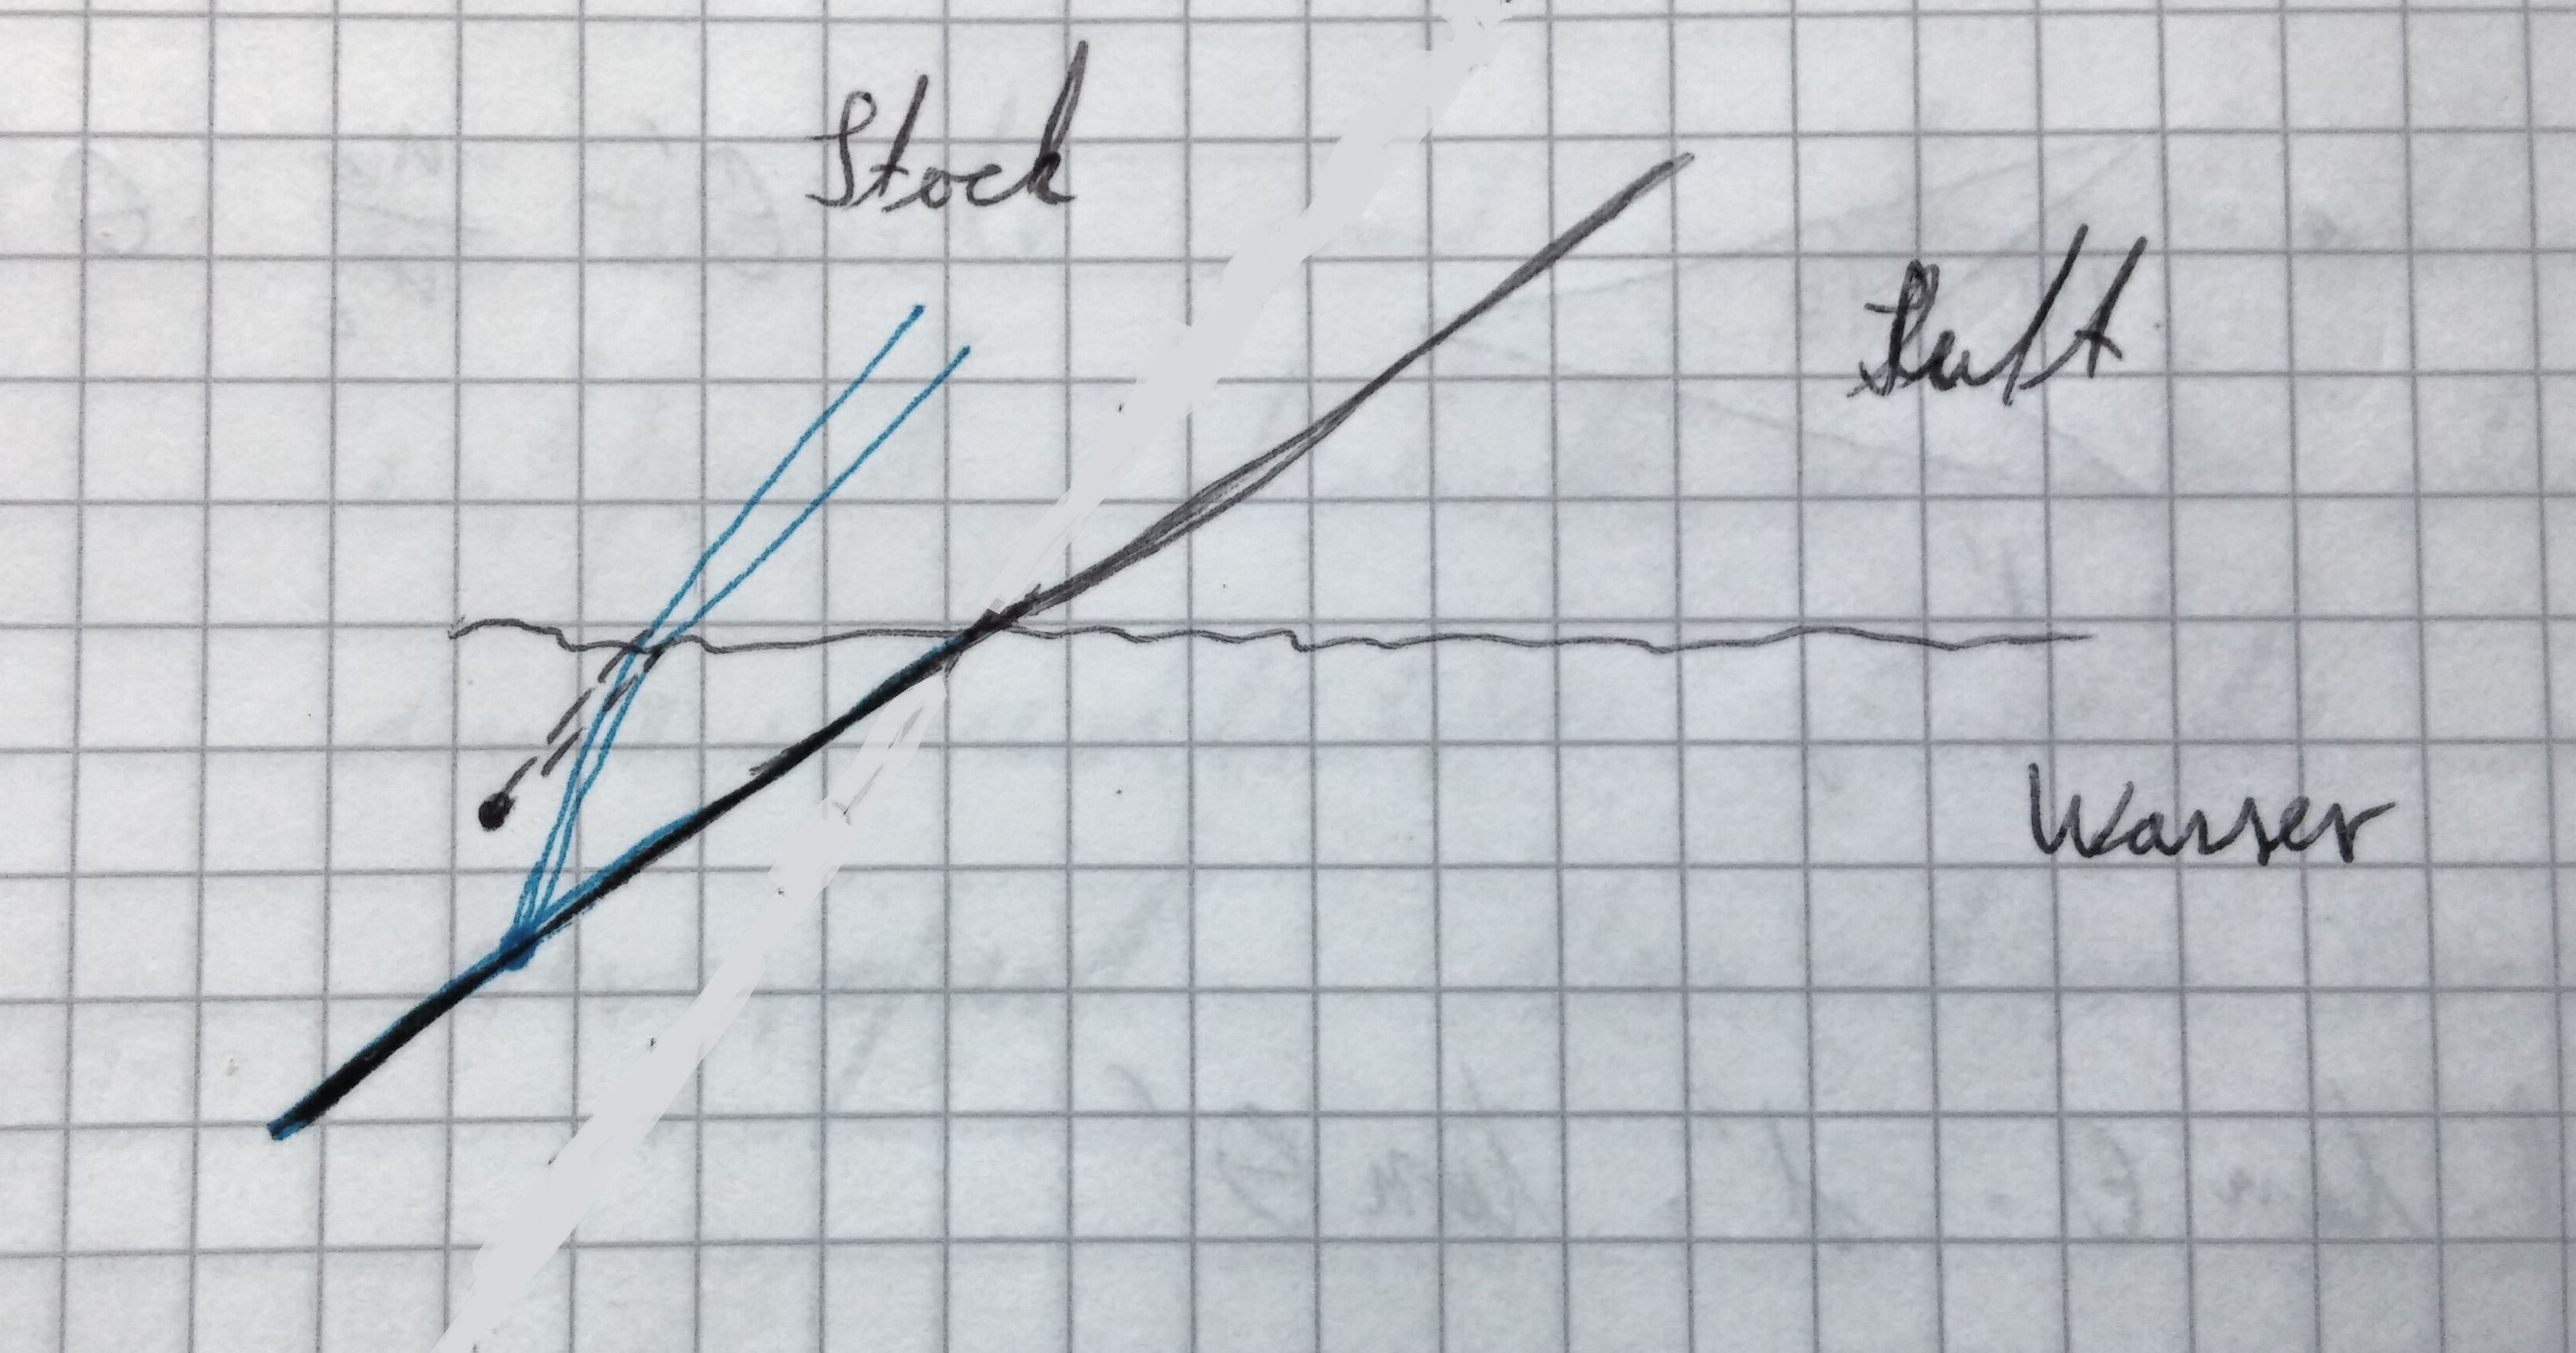
\includegraphics[scale=0.1]{A2_1.jpg}
\end{figure}

Das Auge sieht nur den Strahlenverlauf außerhalb des Wassers und projiziert den Punkt daher an eine höhere Position als er eigentlich ist. Daher hat der Stock einen Knick.


\newpage

\section{Aufgabe 3}

\subsection*{Wasser / Glass}

\begin{figure}[h]
	\centering
	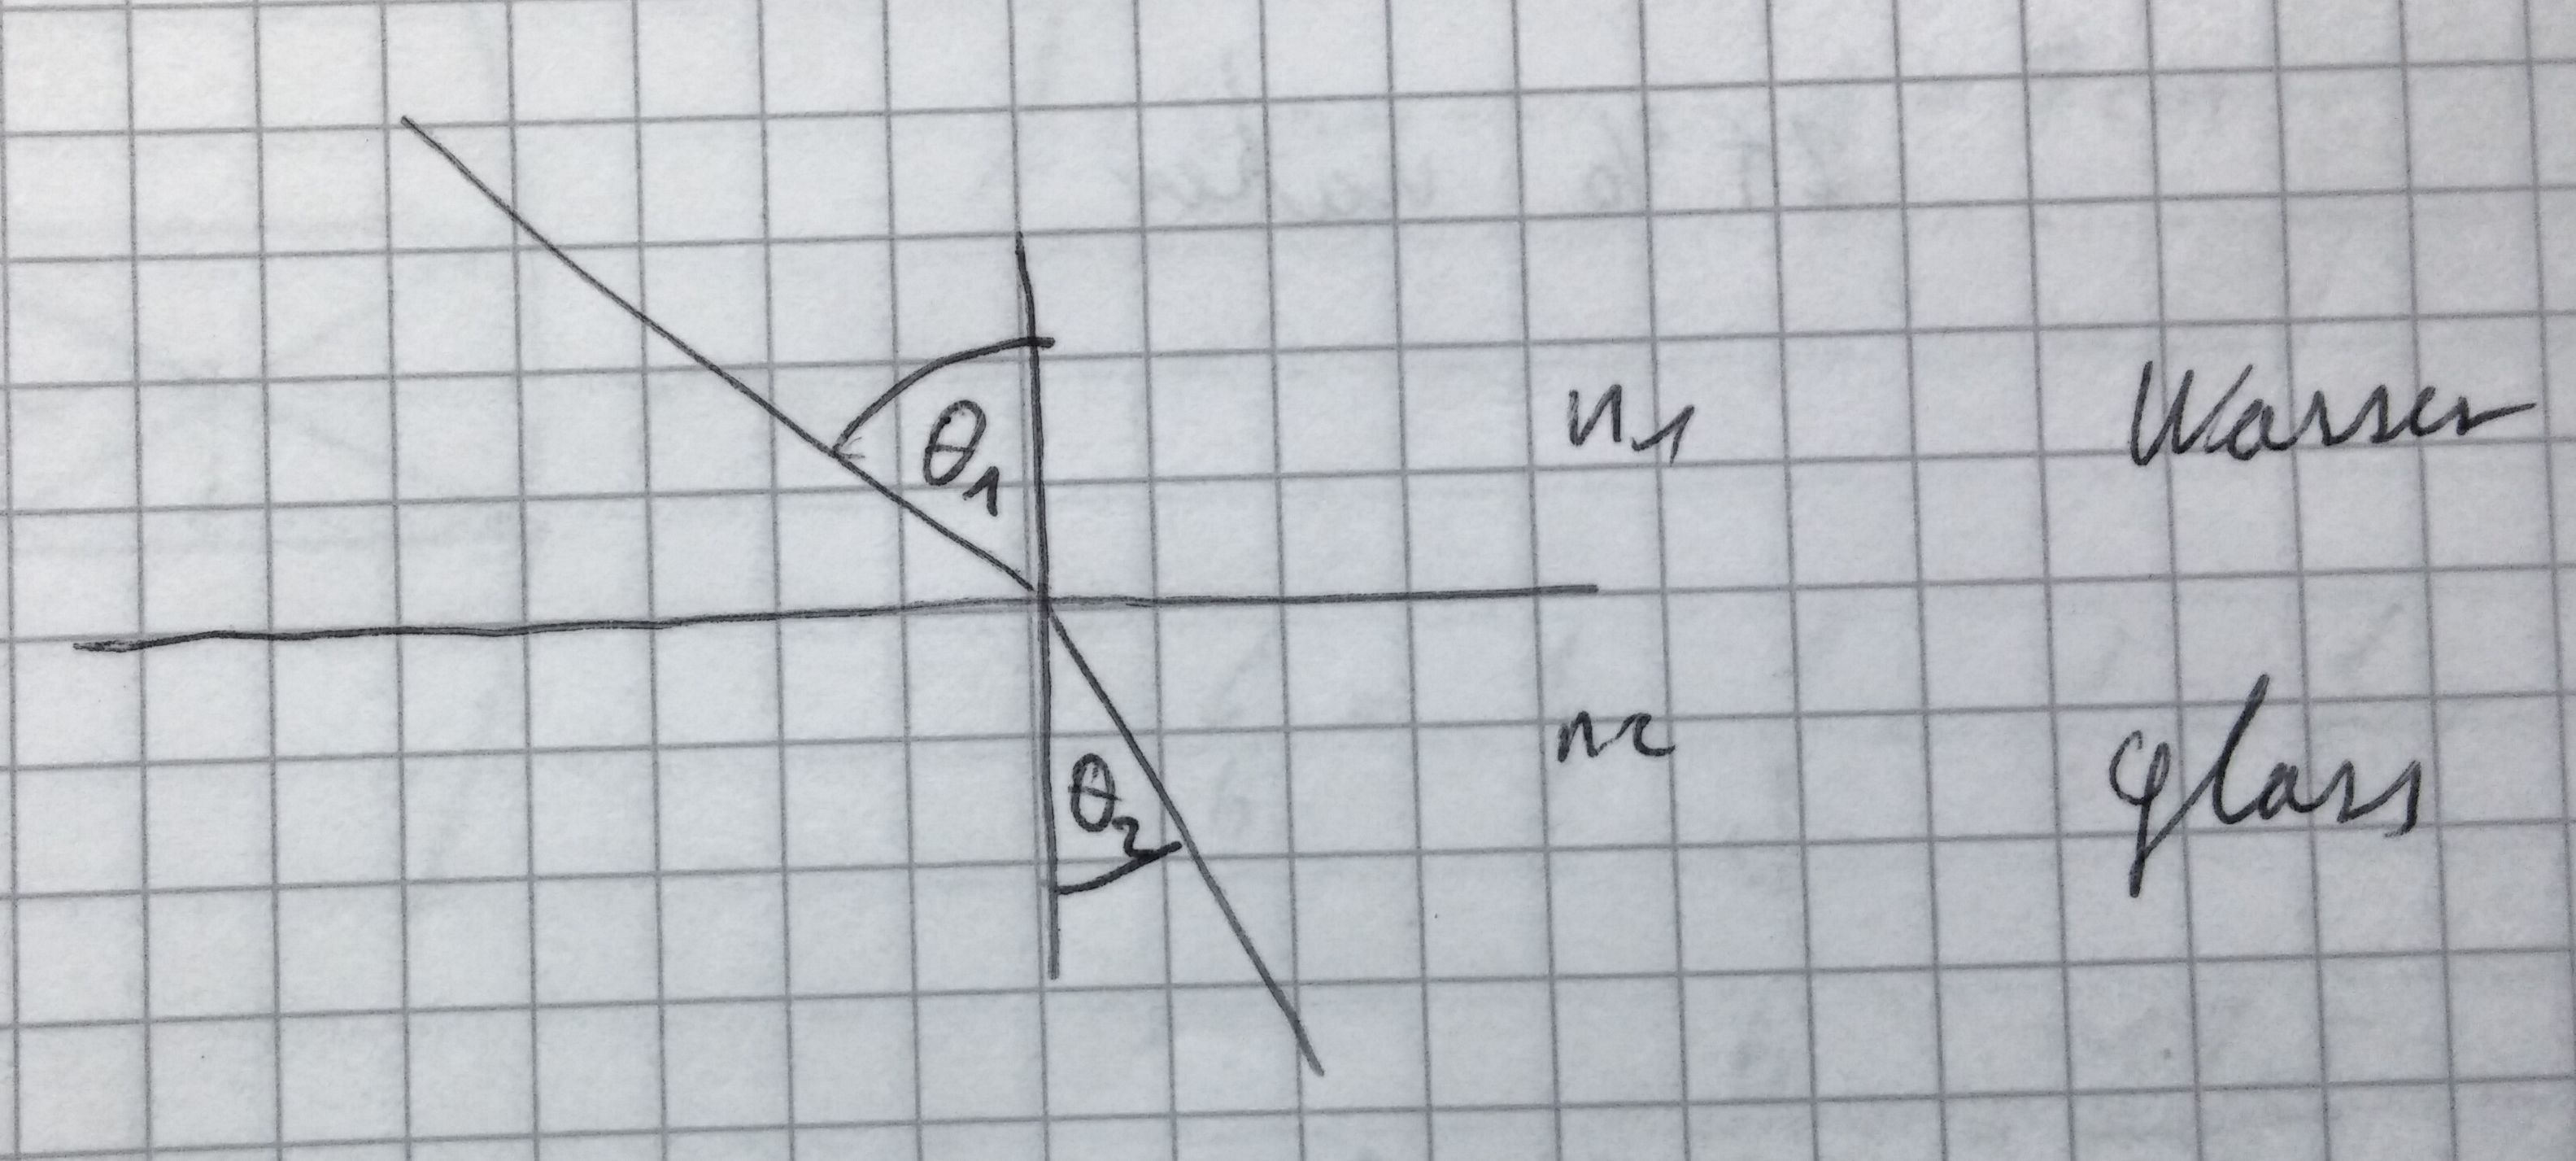
\includegraphics[scale=0.08]{A3_1.jpg}
\end{figure}

\begin{align*}
\frac{4}{3} \cdot \sin(45) &= 1,5 \cdot \sin(\theta_2) \\
\Leftrightarrow \theta_2 &= \arcsin\left(\frac{1,333}{1,5} \cdot \sin(45) \right) = \unit[38,94]{^\circ}
\end{align*}


\subsection*{Glass / Wasser}


\begin{align*}
1,5 \cdot \sin(45) &= 1,33 \cdot \sin(\theta_2) \\
\Leftrightarrow \theta_2 &= \arcsin\left(\frac{1,5}{1,33} \cdot \sin(45) \right) = \unit[52,7]{^\circ}
\end{align*}




\section{Aufgabe 4}

Still missing......

\newpage

\section{Aufgabe 5}


\begin{figure}[h]
	\centering
	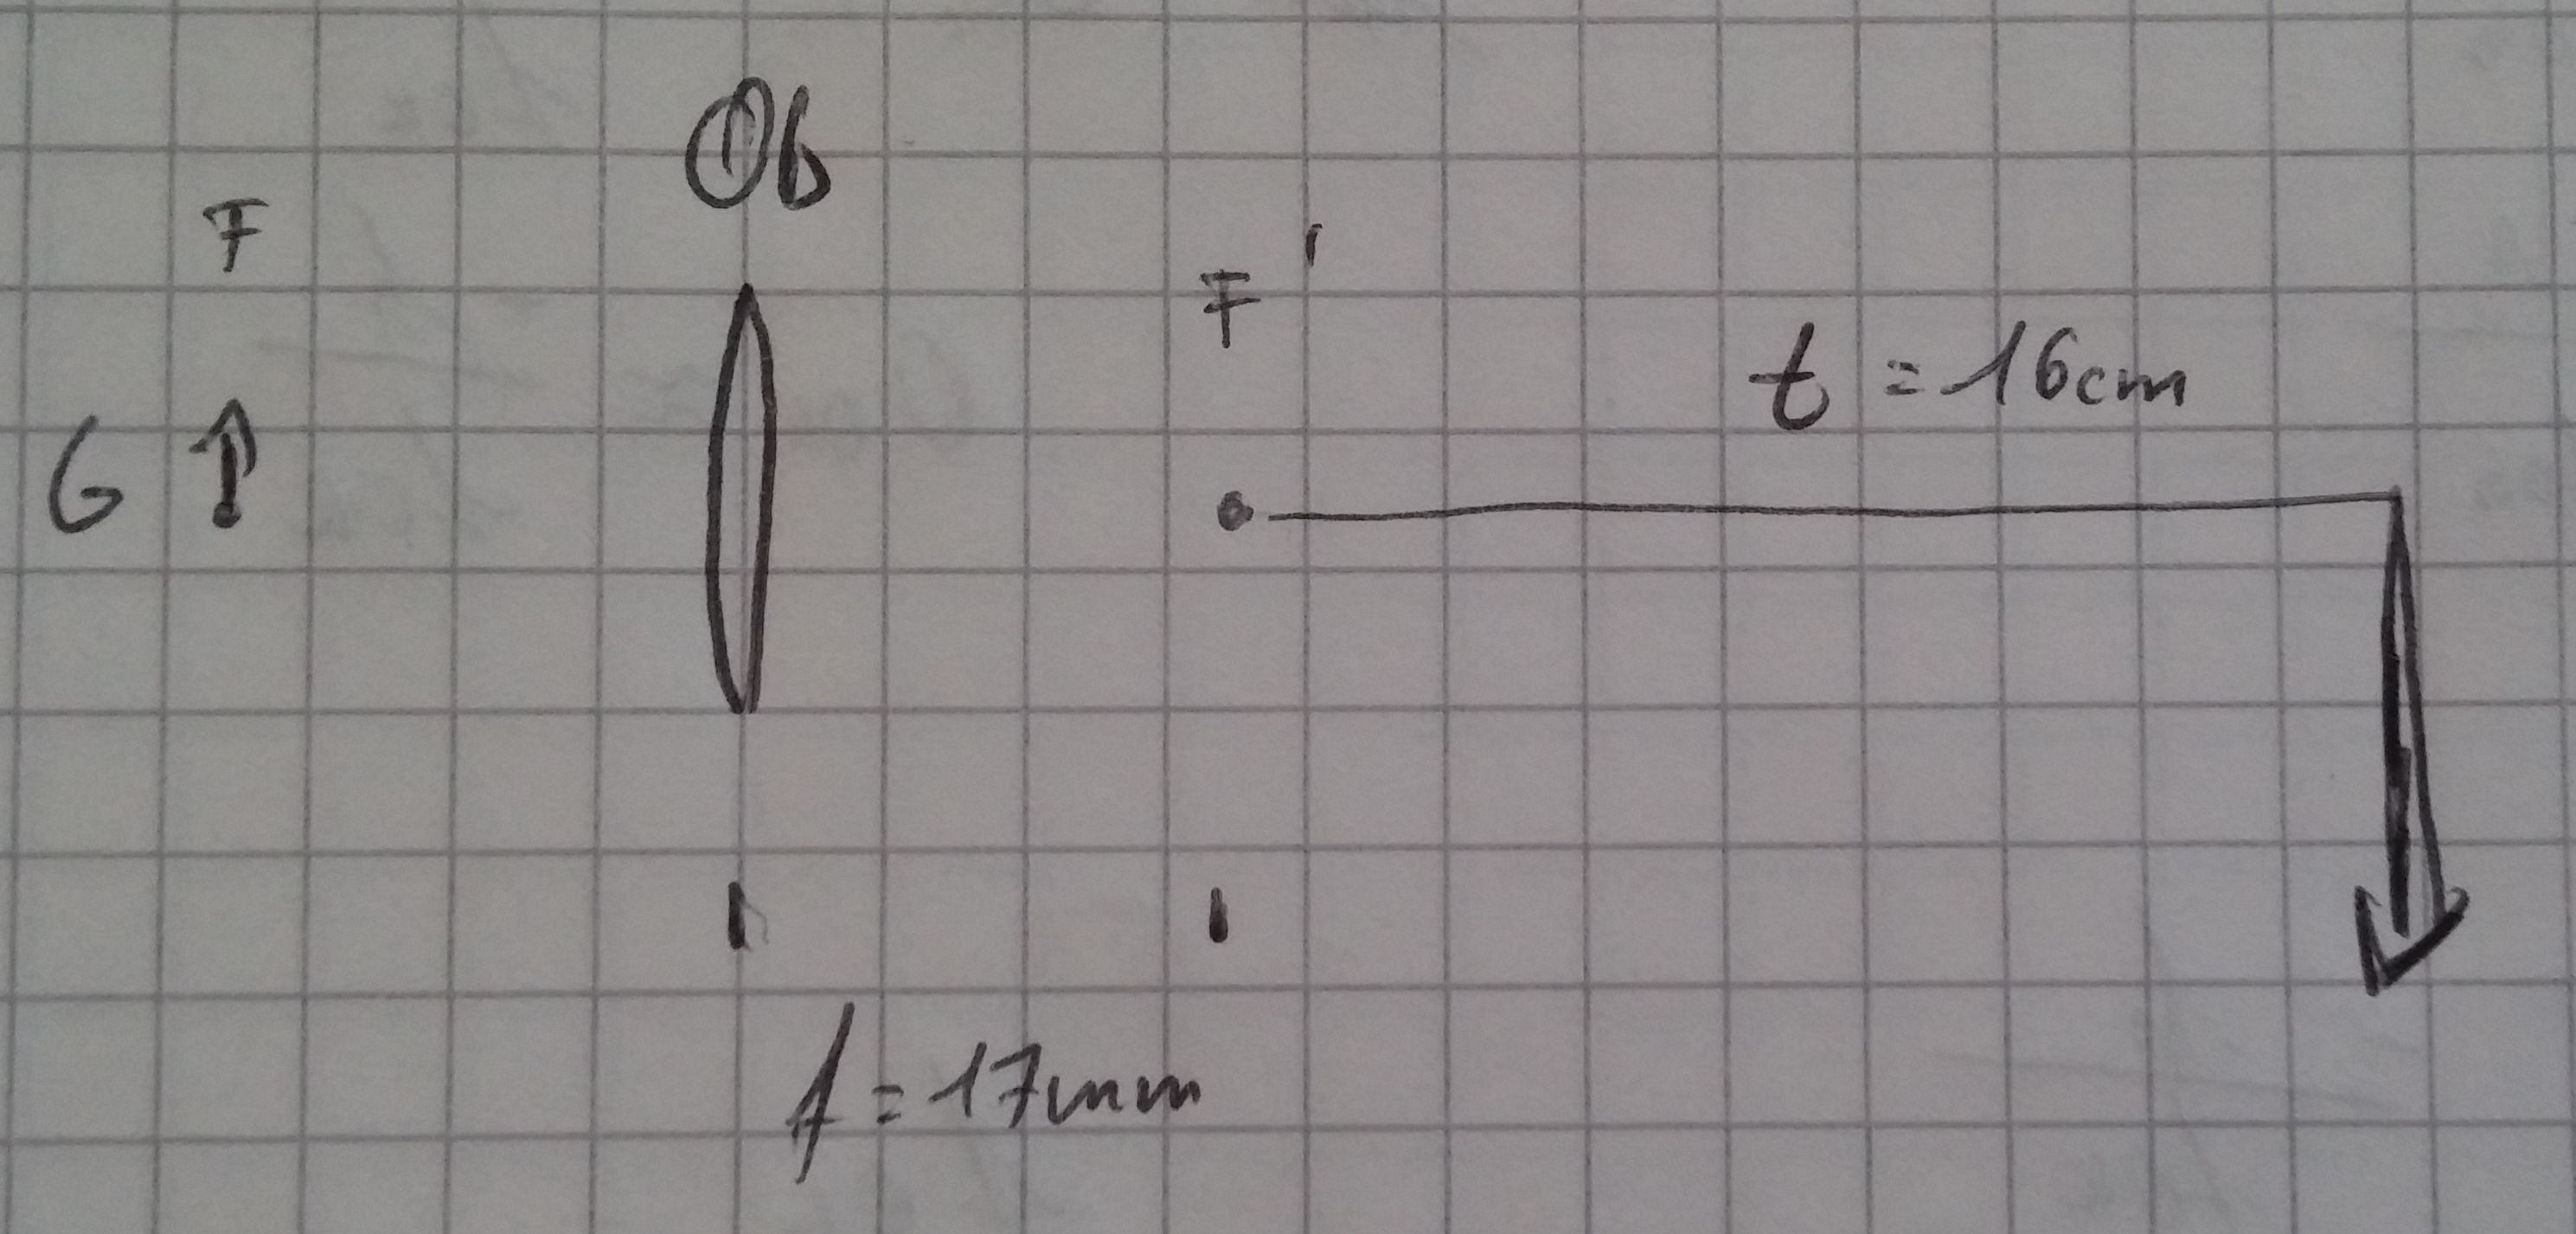
\includegraphics[scale=0.12]{A5_1.jpg}
\end{figure}


\begin{align*}
\theta' &= \frac{n_W}{n_L} \cdot \theta 
\intertext{Wir stellen nun eine Beziehung zur Seite $a$ her:}
a &= d \cdot \tan(\theta) = d' \cdot \tan(\theta') \\
&\approx d \cdot \theta = d' \cdot \theta' \\
d' &= d \cdot \frac{\theta}{\theta'} = \frac{d}{n_W} = \frac{3}{4} \cdot d
\end{align*}

Der Fisch erscheint als um $\unit[25]{\%}$ näher.


\section{Aufgabe 6}

Wir haben einen Radius von $\unit[-10]{cm}$, also eine Brennweite von $\unit[5]{cm}$:

\begin{align*}
\frac{1}{b} &= \frac{1}{f} - \frac{1}{g} = \frac{-1}{5} - \frac{1}{7} = \frac{-12}{35} \\
\Leftrightarrow b &= \frac{-35}{12} = \unit[-3]{cm}
\intertext{Das Bild steht also $\unit[3]{cm}$ hinter dem Spiegel.}
m &= - \frac{b}{g} = - \frac{-3}{7} = 0,42
\intertext{Das Bild ist also verkleinert und aufrecht. Das Bild dazu darf gerne selber gemalt werden.....}
\end{align*}




\section{Aufgabe 7}

Der Knackpunkt ist, das man sich im Bereich von ca einer Brennweite vom Löffel entfernt befindet. Die unterschiedlichen Bereiche des Gesichts haben nun jedes eine (nicht zu vernachlässigende) andere Entfernung vom Löffel. Daher werden die Bereiche unterschiedlich vergrößert und man hat eine Knollnase.


\section{Aufgabe 8}

Wir rechnen wie in Aufgabe 6:

Wir haben einen Radius von $\unit[10]{cm}$, also eine Brennweite von $\unit[5]{cm}$:

\begin{align*}
\frac{1}{b} &= \frac{1}{f} - \frac{1}{g} = \frac{1}{5} - \frac{1}{7} = \frac{2}{35} \\
\Leftrightarrow b &= \frac{35}{2} = \unit[17,5]{cm}
\intertext{Das Bild steht also $\unit[17,5]{cm}$ vor dem Spiegel.}
m &= - \frac{b}{g} = - \frac{17,5}{7} = -2,5
\intertext{Das Bild ist also vergrößert und auf dem Kopf. Das Bild dazu darf gerne selber gemalt werden.....}
\end{align*}


\section{Aufgabe 9}

Ich verweise hierzu auf die in der Mail angehängte und hier eingefügt Erklärung:

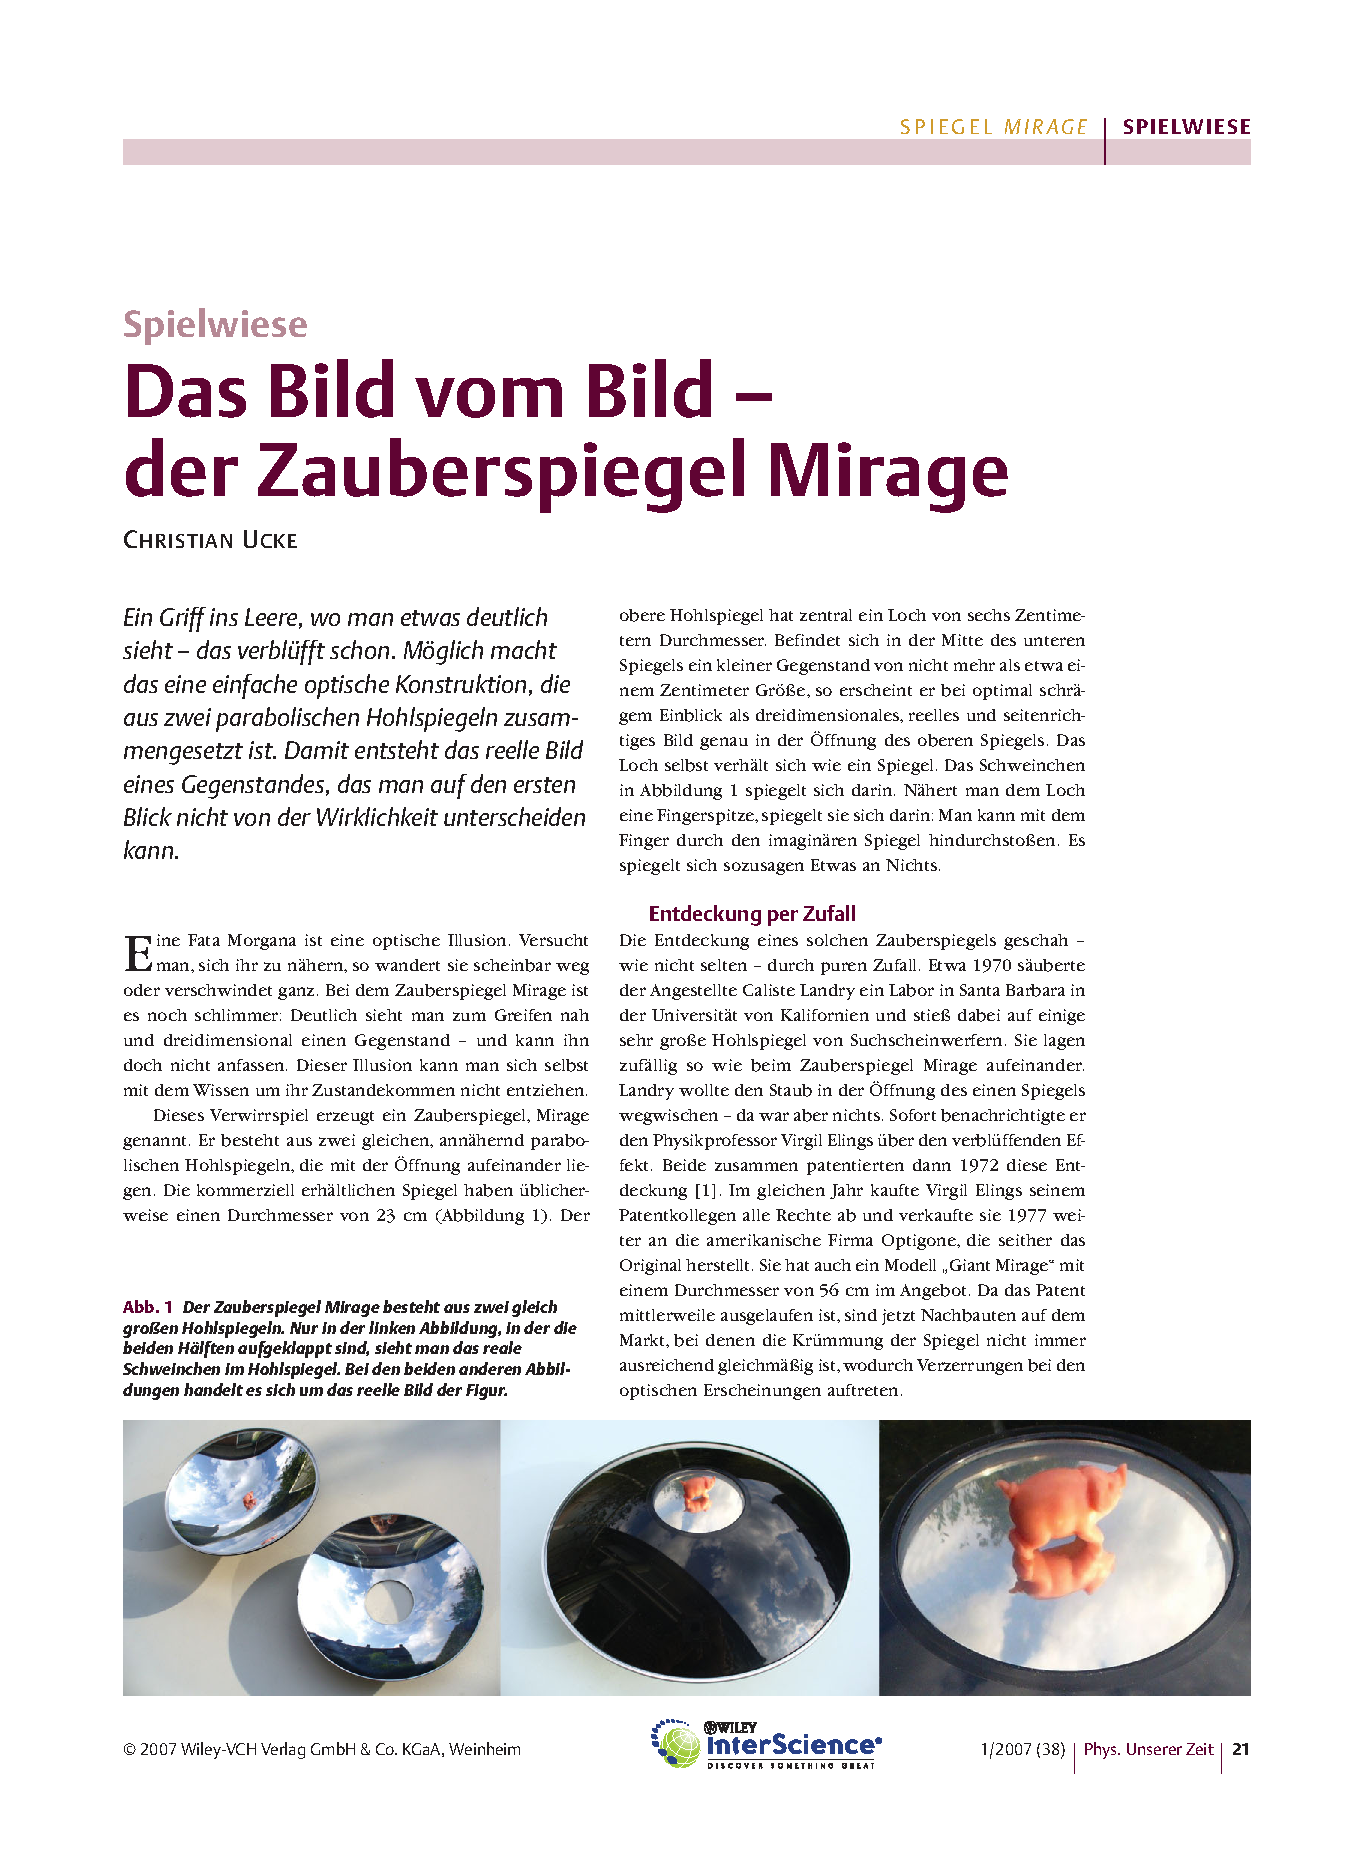
\includepdf[pages={1-3}]{Mirage.pdf}
















\end{document}